\documentclass[10pt]{beamer}

%%%
% PREAMBLE FOR THIS DOC 
%%%
%https://tex.stackexchange.com/questions/68821/is-it-possible-to-create-a-latex-preamble-header
\usepackage{/Users/miw267/Repos/csci246_spring2025/slides/preambles/beamer_preamble_for_CSCI246}



%%% TRY TO RESHOW TOC AT EACH SECTION START (with current section highlighted)
% Reference: https://tex.stackexchange.com/questions/280436/how-to-highlight-a-specific-section-in-beamer-toc
\newcommand\tocforsect[2]{%
  \begingroup
  \edef\safesection{\thesection}
  \setcounter{section}{#1}
  \tableofcontents[#2,currentsection]
  \setcounter{section}{\safesection}
  \endgroup
}


%%%% HERES HOW TO DO IT CORRECTLY
% FIRST IN .STY FILE, DO
%\usetheme[sectionpage=none]{metropolis}
% THEN AT EACH SECTION DO
%\begin{frame}{Outline}
%  \tableofcontents[currentsection]	
%\end{frame}



%\setbeamertemplate{navigation symbols}{}
%\setbeamertemplate{footline}[frame number]{}


%%%
% DOCUMENT
%%%

\begin{document}

%\maketitle

%% Title page frame
%\begin{frame}
%    \titlepage 
%\end{frame}





\title{02/14/2025: Set operations}
\author{CSCI 246: Discrete Structures}
\date{Textbook reference: Sec. 12, Scheinerman}

\begin{frame}
    \titlepage 
\end{frame}


\begin{frame}
\footnotesize 
\begin{mygreenbox}[title=Graded Quiz Pickup]
Quizzes are in the front of the room, grouped into four bins (A-G, H-L, M-R, S-Z) by last name. The quizzes are upside down with your last name on the back. Come find yours before, during, or after class.  Only turn the quiz over if it's yours.
\end{mygreenbox} 
\vfill 

%\begin{myredbox}[title=Announcements]
%
%\begin{itemize}
%\item Wednesday's reading quiz was graded out of 1 point.  45/60 students who took the quiz scored 100\%.
%\item Note: The reading quizzes are equally weighted.  The denominator is typically chosen for convenience.  
%\end{itemize}
%
%\end{myredbox}
%
%\vfill 


\begin{myyellowbox}[title=Today's Agenda]
\begin{itemize}
	\item Reading and problems quizzes (15 mins)
	\item Mini-lecture ($\approx$ 15 mins)
%	%
%	\begin{itemize}
%	\footnotesize 
%	\item Review induction 
%	\end{itemize}
%	%
	\item Group exercises ($\approx$ 20 mins)
\end{itemize}

\end{myyellowbox}
\vfill 

\end{frame}




\begin{frame}
\footnotesize 
%
%\alert{Reminder:} Please write your last name on the back of your page.
%\vfill 
 \begin{mygreenbox}[title=Reading Quiz (Set Operations)]
How many integers in the range 1 to 1000 (inclusive) are divisible by 2 or by 5?  Justify your answer. \textbf{Hint:} Use Proposition 12.4.
\end{mygreenbox}

\vfill 


\begin{myyellowbox}[title=Proposition 12.4 (Scheinerman)]
Let $A$ and $B$ be finite sets.  Then \quad $|A| + |B| = |A \cup B| + |A \cap B|$.
%\[ |A| + |B| = |A \cup B| + |A \cap B|. \]
\end{myyellowbox}
\vfill 

 \begin{myredbox}[title=\text{Problems Quiz (Lists, Factorials, and Intro to Sets)}]

	\begin{minipage}{0.72\textwidth}
	1. A candy shop is preparing two Valentine’s Day  gift bags by selecting sweets from a collection of 100 different types of sweets (including lollipops, truffles, gummies, etc.)   There are many of each of the 100 types of sweets.  The first gift bag should contain 10 candies, each of a different type. The second gift bag should contain 5 candies, each of a different type.  A candy type can appear in both bags, but each bag must have only unique types of candy within it. In how many different ways can the shop fill the two gift bags?
	    \end{minipage}
		\hfill 
	    % Right Column: Image
	    \begin{minipage}{0.26\textwidth}
	        \centering
	        \includegraphics[width=\textwidth]{images/candy_shop} 
	    \end{minipage}
	
\vspace{0.15cm}
2. Prove that the following two sets are equal:
%
\begin{align*}
E &= \set{x \in \mathbb{Z}: x \text{\; is even}}, \text{and} \\
F &= \set{x \in \mathbb{Z}: x=a+b, \text{where $a$ and $b$ are both odd}}
\end{align*}
%
%Note: If we have done an exercise in the past which provides part of the solution, you may write "as we showed in a previous exercise (...)"
\end{myredbox}

\end{frame}


\begin{frame}[standout]
Feedback on Wednesday's Reading Quizzes on Quantifiers
\end{frame} 


\begin{frame}{Scores on Reading Quiz (Quantifiers)}
\begin{figure}
\includegraphics[width=.9\textwidth]{images/reading_quiz_scores}
\caption{Median = 4.0 (100\%)}
\end{figure}	
\vfill 
\footnotesize 
\textit{Rubric:} I used the standard 4-point grading scale for proofs.  (Exception: Due to the existence of participation grades, I am not giving 1 point just for writing something down.)
\end{frame}


\begin{frame}

 \begin{mygreenbox}[title=Reading Quiz (Quantifiers)]
Let $A = \set{x \in \mathbb{Z}: 6|x}$.  Prove that $\forall x \in A, $ x is even.
\end{mygreenbox}
\vfill 
 \begin{myyellowbox}[title=Puzzle]
Evaluate the (partial) student solution below. 
\end{myyellowbox}

\vfill 
 \begin{myredbox}[title=(Partial) Student Solution]

\begin{align}
A = \set{x \in \mathbb{Z}: 6|x} \\
\exists y, \forall x, \; x=6y
\end{align}
\end{myredbox}
\pause 
\vfill 
 \begin{myyellowbox}[title=Comments]
Line 2 in the solution is \texttt{False}. 

\[ \explaintermbrace{there exists}{\exists} y, \explaintermbrace{for all}{\forall} x, \; x=6y \] 
 (No matter what you pick for $y$, 6 times $y$ can't represent all integers).
\end{myyellowbox}

\end{frame}


\begin{frame}{Solution Sketch}
\footnotesize 
 \begin{myyellowbox}[title=General Observation]
The primary issue (even to students who scored 4/4) was \textbf{communication} -- that is structuring the mathematical argument clearly. 
%Note that you can just reuse the old if-then proof template.
\end{myyellowbox}
\vfill 
 \begin{mygreenbox}[title=\text{Solution Using The If-Then Proof Template.}]
\textbf{Proposition.} Let $A = \set{x \in \mathbb{Z}: 6|x}$.  Then $\forall x \in A, $ x is even.

\vspace{0.25cm}

\textbf{Proof.}

\begin{tabularx}{\textwidth}{|L{3cm}|X|}
\hline \textbf{Annotation} & \textbf{Main Text} \\ \hline
 \hlorange{Convert Prop. to ``if-then" form} &  \hlorange{We show that if $x \in A$, then $x$ is even.} \\ \hline
\hlblue{State assumption} & \hlblue{Suppose $x \in A$.} \\ \hline
\hlgreen{Unravel defs.} & \hlgreen{So $6|x$.  That is, there is an integer $c$ such that $x=6c$.} \\ \hline
\hlred{*** The glue ***} & \hlred{We can write $x=6c=2(3c)$.} \\ \hline
 \hlgreen{Unravel defs.} & \hlgreen{So there is an integer $d \red{(=3c)}$ such that $x=2d$. In other words, $2|x$.  } \\ \hline
  \hlblue{State conclusion.} & \hlblue{So, $x$ is even.} \\ \hline
\hline
\end{tabularx}
\end{mygreenbox}
\end{frame}


\begin{frame}[standout]
Notes on set operations
\end{frame}



\begin{frame}{Intuition about set operations}
\footnotesize 
We can build intuition about the set properties by creating an application.
\\
For example, one of the distributive properties is:
\[ A \cap (B \cup C) = (A \cap B) \cup (A \cap C). \]

Suppose we work for Rosauers and we are studying how likely customers are to make a purchase in different parts of the store.  Let  
\begin{itemize}
\item $P$: The set of Rosauers customers who made a purchase. 
\item $R$: The set of Rosauers customers who were shopping for roses.
\item $C$: The set of Rosauers customers who were shopping for candy.
\end{itemize}

Then
\[ (R \cup C)  \cap P \explaintermbrace{commutative}{=}  P \cap (R \cup C) \explaintermbrace{distributive }{=} (P \cap R) \cup (P \cap C). \]
This says that the set of Rousauers customers who were shopping for roses or candy and made a purchase is the same as the set of Rosauers customers who were shopping for roses and made a purchase combined with the set of Rosauers customers who were shopping for candy and made a purchase.
	
\end{frame}


\begin{frame}{Why set operations matter}
	
\textbf{Question:} Why should we care about the the properties of set operations?  Aren't they obvious (as the previous slide might suggest)? \\
\vfill 
\textbf{Answer:} Sometimes it's easier to do things one way than another. Today's reading quiz is a great example. \\

\end{frame}

\begin{frame}
\footnotesize 
 \begin{mygreenbox}[title=Reading Quiz (Set Operations)]
How many integers in the range 1 to 1000 (inclusive) are divisible by 2 or by 5?  Justify your answer.
\end{mygreenbox}

\vfill 
 \begin{myredbox}[title=Sketch of Solution]
Let
%
\begin{align*}
A &\defeq \set{x \in \mathbb{Z} : 2|x} \\
B &\defeq \set{x \in \mathbb{Z} : 5|x} 
\end{align*}
%
We want $|A \cup B|$.  That's hard to calculate. \\

However, we have
\begin{align*}
|A| &= 500 && \scripttext{(by skip counting)} \\
|B| &= 200 && \scripttext{(by skip counting)} \\
|A \cap B| &= \bigg| \set{x \in \mathbb{Z} : 10|x} \bigg| = 100 && \scripttext{(by skip counting)} 
\end{align*}

Now we apply the identity to find
\begin{align*}
|A \cup B|  &= |A| + |B| - |A \cap B| \\
			&= 500 + 200 - 100 = 600
\end{align*}

\end{myredbox}


\end{frame}

\begin{frame}{Intuition: Avoid double-counting}

\begin{myyellowbox}[title=Proposition 12.4 (Scheinerman)]
Let $A$ and $B$ be finite sets.  Then %\quad $|A| + |B| = |A \cup B| + |A \cap B|$.
\[ |A| + |B| = |A \cup B| + |A \cap B|. \]
\end{myyellowbox}
\vfill 

\begin{center}
\includegraphics[width=.4\textwidth]{images/double_counting.png}	
\end{center}
	
\end{frame}

\begin{frame}{Application: Database management}
\footnotesize 
One application of set theory in computer science is in \textbf{database management systems} (DBMS), particularly in \textbf{SQL query optimization}.
\vfill 

\begin{mygreenbox}[title=Example]
Imagine a company has two database tables:

\begin{itemize}
\item \textbf{Customers} (Set $C$): Contains all registered customers.
\item \textbf{Orders} (Set $O$): Contains all customer orders.
\end{itemize}

A database query like:
\vspace{-.25cm}
\begin{center}
\includegraphics[width=.6\textwidth]{images/sql_query.png}	
\end{center}
\vspace{-.25cm}
is using the set difference $C-O$ to find customers who have never placed an order.
\end{mygreenbox}
\vfill

\begin{myyellowbox}[title=Key Set Operations in Databases]
\begin{itemize}
\item  Union ($A \cup B$)  $\to$ \texttt{UNION} in SQL (Combining results from multiple queries)
\item  Intersection ($A \cap B$)  $\to$ \texttt{INTERSECT} in SQL  (Finding common data between queries)
\item  Set Difference ($A - B$)  $\to$ \texttt{EXCEPT}  or \texttt{NOT IN} in SQL (Finding items in one table but not the other)	
\end{itemize}
\end{myyellowbox}


\end{frame}


\begin{frame}[standout]
Q\&A on the Group Exercises for Quantifiers
\end{frame}


\begin{frame}
\footnotesize
Group 1: ethan.johnson18,joseph.triem,jett.girard\\
Group 2: carsten.brooks,samuel.rollins,pendleton.johnston\\
Group 3: william.elder1,aaron.loomis,delaney.rubb\\
Group 4: owen.obrien,julia.larsen,alexander.goetz\\
Group 5: evan.schoening,griffin.short,jacob.ruiz1\\
Group 6: adam.wyszynski,ryan.barrett2,caitlin.hermanson\\
Group 7: justice.mosso,peyton.trigg,evan.barth\\
Group 8: colter.huber,yebin.wallace,james.brubaker\\
Group 9: jonas.zeiler,jeremiah.mackey,sarah.periolat\\
Group 10: jada.zorn,timothy.true,jakob.kominsky\\
Group 11: devon.maurer,michael.oswald,mason.barnocky\\
Group 12: connor.mizner,bridger.voss,carver.wambold\\
Group 13: matthew.nagel,nolan.scott1,tristan.nogacki\\
Group 14: zeke.baumann,lucas.jones6,peter.buckley1\\
Group 15: joseph.mergenthaler,micaylyn.parker,derek.price4\\
Group 16: connor.yetter,jacob.ketola,blake.leone\\
Group 17: samuel.hemmen,luka.derry,john.fotheringham\\
Group 18: jack.fry,conner.reed1,connor.graville\\
Group 19: jacob.shepherd1,luke.donaldson1,erik.moore3\\
Group 20: cameron.wittrock,tyler.broesel,lynsey.read\\
Group 21: samuel.mosier,emmeri.grooms,reid.pickert\\
Group 22: kaden.price,anthony.mann,alexander.knutson\\\end{frame}


\begin{frame}{Group Exercises: Set Operations}

\footnotesize 
\begin{enumerate}
	\item Let $A=\set{1,2,3,4,5}$ and $B=\set{4,5,6,7}$. Please compute (a) $A \cup B$, (b) $A \cap B$, (c) $A - B$, (d) $B-A$, (e) $A \, \triangle \, B$, (f) $A \times B$, and (g)  $B \times A$.
%    \begin{itemize}
%        \item[a.] $A \cup B$.
%        \item[b.] $A \cap B$.
%        \item[c.] $A - B$.
%        \item[d.] $B-A$.
%        \item[e.] $A \, \triangle \, B$.
%        \item[f.] $A \times B$.
%        \item[g.] $B \times A$.
    % \end{itemize}
    \item The distributive properties for sets are 
    \[ A \cup (B \cap C) = (A \cup B) \cap (A \cup C), \qquad \text{and} \qquad  A \cap (B \cup C) = (A \cap B) \cup (A \cap C). \]
    The Venn diagram below illustrates the first distributive property. Make a Venn diagram to illustrate the second distributive property.
    \begin{center}
    \includegraphics[width=.6\textwidth]{images/set_distributive_property}
    \end{center} 
    \item Prove that the first identity in \#2 holds.  Hint: You may want to refer back to Theorem 7.2.
\end{enumerate}
\end{frame}

\begin{frame}{Solution to Group Exercise \#1 (a-e) }

\textbf{Problem.} Let $A=\set{1,2,3,4,5}$ and $B=\set{4,5,6,7}$. Please compute (a.) $A \cup B$, (b.) $A \cap B$, (c.) $A - B$, (d.) $B-A$, and (e.) $A \, \triangle \, B$.\\
\vfill 
\textbf{Solution.}
   \begin{itemize}
        \item[(a.)] $A \cup B = \set{1,2,3,4,5,6,7}$.
        %\textit{Explanation.} The union is set of elements in either $A$ or $B$.
        \item[(b.)] $A \cap B = \set{4,5}$.  %\textit{Explanation.} The intersection is set of elements in both $A$ and $B$.
        \item[(c.)] $A - B = \set{1,2,3}$.
        \item[(d.)] $B-A = \set{6,7}$.
        \item[(e.)] $A \, \triangle \, B = \set{1,2,3,6,7}$. [Note:  $A \, \triangle \, B = (A-B) \cup (B-A)$.]
    \end{itemize}

\end{frame}

\begin{frame}{Solution to Group Exercise \#1 (f-g) }

\footnotesize 
\textbf{Problem.} Let $A=\set{1,2,3,4,5}$ and $B=\set{4,5,6,7}$. Please compute (f.) $A \times B$ and (g.)  $B \times A$.\\

\textbf{Solution.}
   \begin{itemize}
        \item[(f.)]    
        \begin{align*}
	A \times B = \bigg\{ & (1,4),(1,5),(1,6),(1,7), \\
	& (2,4),(2,5),(2,6),(2,7), \\
& (3,4),(3,5),(3,6),(3,7), \\
 & (4,4),(4,5),(4,6),(4,7), \\
& (5,4),(5,5),(5,6),(5,7)    \bigg\}    	
    \end{align*}
        \item[(g.)]    
        \begin{align*}
	B \times A = \bigg\{ & (4,1),(4,2),(4,3),(4,4), (4,5) \\
 & (5,1),(5,2),(5,3),(5,4), (5,5) \\
 & (6,1),(6,2),(6,3),(6,4), (6,5) \\
& (7,1),(7,2),(7,3),(7,4), (7,5)   \bigg\}   
    \end{align*}
    \end{itemize}
    
\end{frame}


\begin{frame}{Solution to Group Exercise \#2 }
\footnotesize 
\textbf{Problem.} The distributive properties for sets are 
    \[ A \cup (B \cap C) = (A \cup B) \cap (A \cup C), \qquad \text{and} \qquad  A \cap (B \cup C) = (A \cap B) \cup (A \cap C). \]
 Make a Venn diagram to illustrate the second distributive property.
 \vfill 
 \textbf{Solution.}
	\scalebox{0.5}{  % Scale everything down 
        \begin{tabular}{ccc}   % Create a 2x3 grid
        % First Venn Diagram
        \Huge \textbf{$A$} &         \Huge \textbf{$B \cup C$}  &        \Huge \textbf{$A \cap (B \cup C)$} \\
        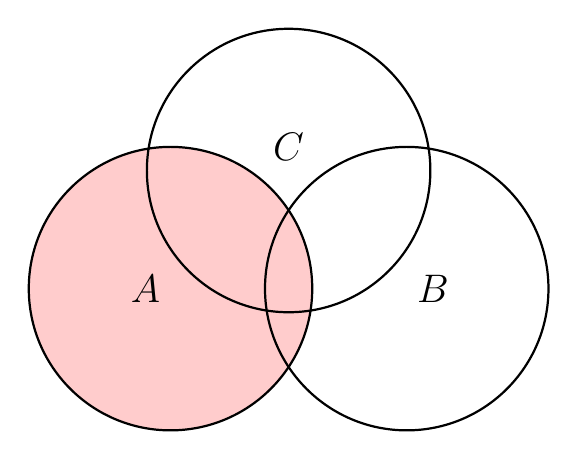
\begin{tikzpicture}
             \fill[red!20] (-1.5,0) circle (1.8);  % Set A (shaded)
            \draw[thick] (-1.5,0) circle (1.8) node[left] {\Large \( A \)};
            \draw[thick] (1.5,0) circle (1.8) node[right] {\Large \( B \)};
            \draw[thick] (0,1.5) circle (1.8) node[above] {\Large \( C \)};
        \end{tikzpicture}
        &
        % Second Venn Diagram
        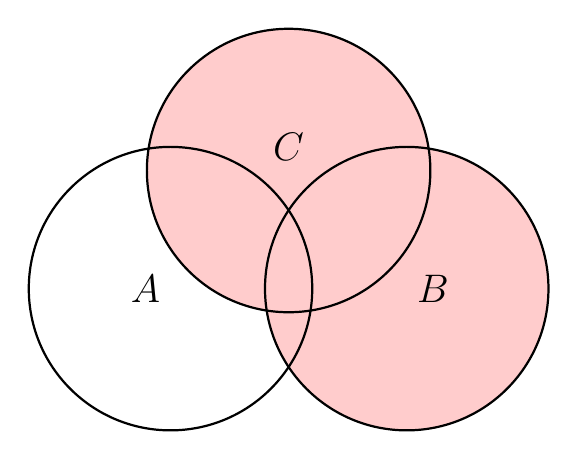
\begin{tikzpicture}
           \fill[red!20] (1.5,0) circle (1.8);  % Set B (shaded)
            \fill[red!20] (0,1.5) circle (1.8);  % Set C (shaded)
            \draw[thick] (-1.5,0) circle (1.8) node[left] {\Large \( A \)};
            \draw[thick] (1.5,0) circle (1.8) node[right] {\Large \( B \)};
            \draw[thick] (0,1.5) circle (1.8) node[above] {\Large \( C \)};
        \end{tikzpicture}
        &
        % Third Venn Diagram
        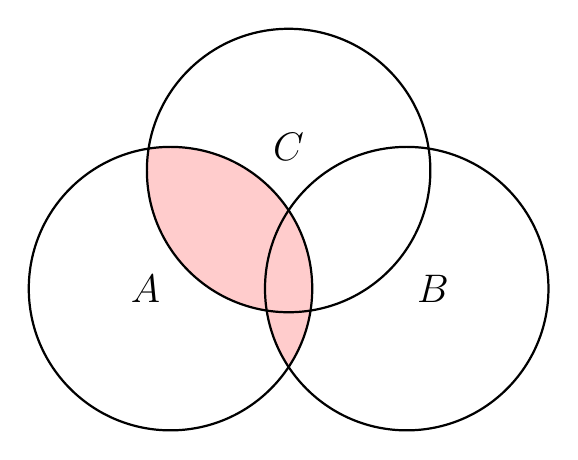
\begin{tikzpicture}
	         % Shade A ∩ (B ∪ C)
	        \begin{scope}
	            \clip (-1.5,0) circle (1.8); % Clip to A
	            \fill[red!20] (1.5,0) circle (1.8); % Fill B
	            \fill[red!20] (0,1.5) circle (1.8); % Fill C
	        \end{scope}
        
            \draw[thick] (-1.5,0) circle (1.8) node[left] {\Large \( A \)};
            \draw[thick] (1.5,0) circle (1.8) node[right] {\Large \( B \)};
            \draw[thick] (0,1.5) circle (1.8) node[above] {\Large \( C \)};
        \end{tikzpicture}
        \\
        & & \\
         \Huge \textbf{$A \cap B$} &         \Huge \textbf{$A \cap C$}  &        \Huge \textbf{$(A \cap B) \cup (A \cap C)$} \\
        % Fourth Venn Diagram
        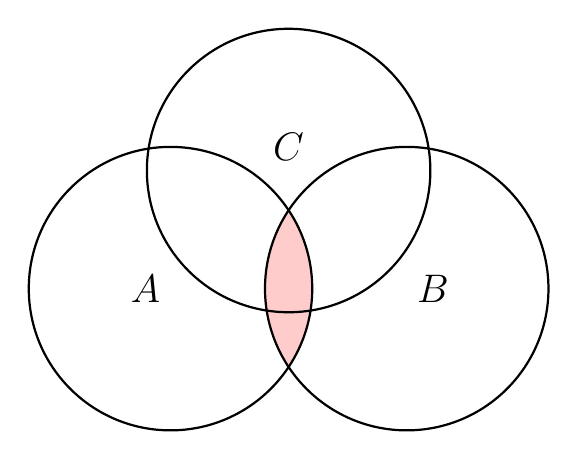
\begin{tikzpicture}
            % Shade A ∩ B
	        \begin{scope}
	            \clip (-1.5,0) circle (1.8); % Clip to A
	            \fill[red!20] (1.5,0) circle (1.8); % Fill B
	        \end{scope}
	        
            \draw[thick] (-1.5,0) circle (1.8) node[left] {\Large \( A \)};
            \draw[thick] (1.5,0) circle (1.8) node[right] {\Large \( B \)};
            \draw[thick] (0,1.5) circle (1.8) node[above] {\Large \( C \)};
        \end{tikzpicture}
        &
        % Fifth Venn Diagram
        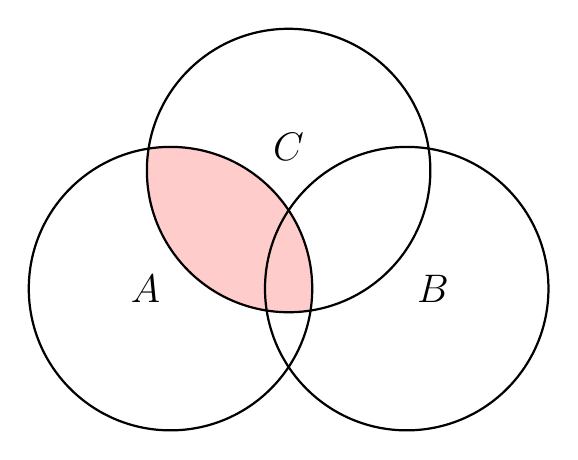
\begin{tikzpicture}
             % Shade A ∩ C
	        \begin{scope}
	            \clip (-1.5,0) circle (1.8); % Clip to A
	            \fill[red!20] (0,1.5) circle (1.8); % Fill C
	        \end{scope}
	        
            \draw[thick] (-1.5,0) circle (1.8) node[left] {\Large \( A \)};
            \draw[thick] (1.5,0) circle (1.8) node[right] {\Large \( B \)};
            \draw[thick] (0,1.5) circle (1.8) node[above] {\Large \( C \)};
        \end{tikzpicture}
        &
        % Sixth Venn Diagram
        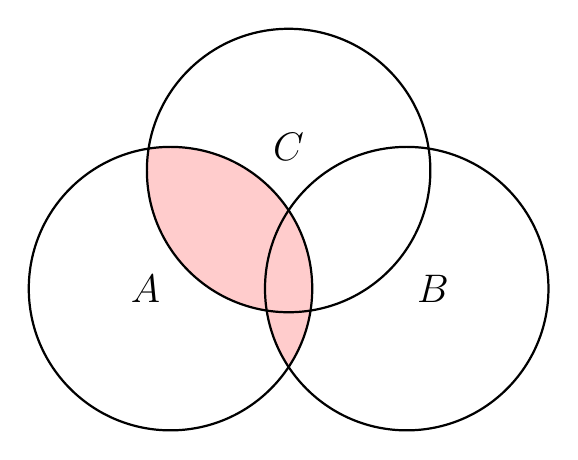
\begin{tikzpicture}
	        \begin{scope}
	            \clip (-1.5,0) circle (1.8); % Clip to A
	            \fill[red!20] (1.5,0) circle (1.8); % Fill B
	            \fill[red!20] (0,1.5) circle (1.8); % Fill C
	        \end{scope}
        
            \draw[thick] (-1.5,0) circle (1.8) node[left] {\Large \( A \)};
            \draw[thick] (1.5,0) circle (1.8) node[right] {\Large \( B \)};
            \draw[thick] (0,1.5) circle (1.8) node[above] {\Large \( C \)};
        \end{tikzpicture}
    \end{tabular}
    }
\end{frame}


\begin{frame}{Solution to Group Exercise \#3 }
\footnotesize 
\textbf{Problem.} The distributive properties for sets are 
    \[ A \cup (B \cap C) = (A \cup B) \cap (A \cup C), \qquad \text{and} \qquad  A \cap (B \cup C) = (A \cap B) \cup (A \cap C). \]
Prove that the first identity above holds.  Hint: You may want to refer back to Theorem 7.2.	

\textbf{Solution.}

\begin{align*}
A \cup (B \cap C) &= \set{x: x \in A \text{ or } x \in B \cap C} && \scripttext{(by def. union $\cup$)} \\
&= \set{x: x \in A \text{ or } (x \in B \text{ and }  x \in C) } && \scripttext{(by def. intersection $\cap$)} \\
&= \set{x: (x \in A \text{ or } x \in B) \text{ and }  (x \in A \text{ or } x \in C) } && \scripttext{(by distributive prop.; Thm 7.2)} \\
&= \set{x: (x \in A \cup B) \text{ and }  (x \in A \cup C)} && \scripttext{(by def. union $\cup$)} \\
&= (A \cup B) \cap (A \cup C) && \scripttext{(by def. intersection $\cap$)}
\end{align*}

\textbf{Remark.} We used the distributive property for \textit{Boolean Algebra} (from Theorem 7.2) to prove the distributive property for \textit{sets}.
\end{frame}


\end{document}
